%% This is the ctufit-thesis example file. It is used to produce theses
%% for submission to Czech Technical University, Faculty of Information Technology.
%%
%% This is version 1.3.10, built 27. 2. 2025.
%% 
%% Get the newest version from
%% https://gitlab.fit.cvut.cz/theses-templates/FITthesis-LaTeX
%%
%%
%% Copyright 2024, Tomas Novacek
%% Copyright 2021, Eliska Sestakova and Ondrej Guth
%%
%% This work may be distributed and/or modified under the
%% conditions of the LaTeX Project Public License, either version 1.3
%% of this license or (at your option) any later version.
%% The latest version of this license is in
%%  https://www.latex-project.org/lppl.txt
%% and version 1.3 or later is part of all distributions of LaTeX
%% version 2005/12/01 or later.
%%
%% This work has the LPPL maintenance status `maintained'.
%%
%% The current maintainer of this work is Tomas Novacek.
%% Alternatively, submit bug reports to the tracker at
%% https://gitlab.fit.cvut.cz/theses-templates/FITthesis-LaTeX/issues
%%
%%

% arara: xelatex
% arara: biber
% arara: xelatex
% arara: xelatex

%%%%%%%%%%%%%%%%%%%%%%%%%%%%%%%%%%%%%%%%%
% CLASS OPTIONS
% language: czech/english/slovak
% thesis type: bachelor/master/dissertation
% colour: bw for black&white OR no option for default colour scheme
% electronic (oneside) or printed (twoside), twoside is default
% paragraph - if passed, this optional argument sets paragraphs as the deepest level of headers, styles it, numbers it and adds it to Table of Content. Use with care! Normally, it is considered unwise to use it, since its too deep.
%%%%%%%%%%%%%%%%%%%%%%%%%%%%%%%%%%%%%%%%%
\documentclass[english,bachelor,unicode,oneside]{ctufit-thesis}

%%%%%%%%%%%%%%%%%%%%%%%%%%%%%%%%%%
% FILL IN THIS INFORMATION
%%%%%%%%%%%%%%%%%%%%%%%%%%%%%%%%%%
\ctufittitle{Efficiency and utilization of Vector Packet Processing in high-speed networks} % replace with the title of your thesis
\ctufitauthorfull{Ondřej Slavík} % replace with your full name (first name(s) and then family name(s) / surname(s)) including academic degrees
\ctufitauthorsurnames{Slavík} % replace with your surname(s) / family name(s)
\ctufitauthorgivennames{Ondřej} % replace with your first name(s) / given name(s)
\ctufitsupervisor{Ing.\,Jan Fesl,\,Ph.D.} % replace with name of your supervisor/advisor (include academic degrees)
\ctufitdepartment{Department of Computer Systems} % replace with the department of your defence
\ctufityear{2025} % replace with the year of your defence
\ctufitdeclarationplace{Prague} % replace with the place where you sign the declaration
\ctufitdeclarationdate{\today} % replace with the date of signature of the declaration
\ctufitabstractCZE{Tato bakalářská práce se zabývá efektivitou a využitím frameworku Vector Packet Processing (VPP) ve vysokorychlostních sítích. Cílem je experimentálně porovnat jeho výkon při zpracování síťových paketů s tradičním síťovým stackem v jádře operačního systému. Práce nejprve představuje teoretické základy VPP a popisuje jeho architekturu. V praktické části jsou navrženy a realizovány testovací scénáře pro porovnání obou řešení. Výsledky ukazují, že VPP dosahuje výrazně vyšší propustnosti, a zároveň i nižší latence a lepší energetické efektivity, zejména při vyšších přenosových rychlostech.}
\ctufitabstractENG{This bachelor’s thesis focuses on the efficiency and utilization of the Vector Packet Processing (VPP) framework in high-speed networks. The aim is to experimentally compare its packet processing performance with the traditional kernel-based networking stack. The thesis first introduces the theoretical foundations of VPP and its architecture. In the practical part, test scenarios are designed and executed to evaluate and compare both solutions. The results show that VPP achieves significantly higher throughput, along with lower latency and better energy efficiency, particularly at higher transmission speeds.}
\ctufitkeywordsCZE{vector packet processing, data plane development kit, síťové měření, energetická efektivita, síťový stack Linuxu}
\ctufitkeywordsENG{vector packet processing, data plane development kit, network benchmark, energy efficiency, Linux network stack}
%%%%%%%%%%%%%%%%%%%%%%%%%%%%%%%%%%
% END FILL IN
%%%%%%%%%%%%%%%%%%%%%%%%%%%%%%%%%%

%%%%%%%%%%%%%%%%%%%%%%%%%%%%%%%%%%
% CUSTOMIZATION of this template
% Skip this part or alter it if you know what you are doing.
%%%%%%%%%%%%%%%%%%%%%%%%%%%%%%%%%%

\RequirePackage{iftex}[2020/03/06]
\iftutex % XeLaTeX and LuaLaTeX
    \RequirePackage{ellipsis}[2020/05/22] %ellipsis workaround for XeLaTeX
\else
    \errmessage{Only compilation with XeLaTeX or LuaLaTeX is allowed}
    \stop
\fi

% hyperlinks
\hypersetup{
    pdfpagelayout=TwoPageRight,
    colorlinks=false,
    allcolors=decoration,
    pdfborder={0 0 0.1}
}

% uncomment the following to hide all hyperlinks
%\hypersetup{hidelinks}

% uncomment the following to change the colour of all hyperlinks to CTU blue
%\hypersetup{allbordercolors=decoration}

\RequirePackage{pdfpages}[2020/01/28]

%%%%%%%%%%%%%%%%%%%%%%%%%%%%%%%%%%
% CUSTOMIZATION of this template END
%%%%%%%%%%%%%%%%%%%%%%%%%%%%%%%%%%


%%%%%%%%%%%%%%%%%%%%%%
% DEMO CONTENTS SETTINGS
% You may choose to modify this part.
%%%%%%%%%%%%%%%%%%%%%%
\usepackage{dirtree}
\usepackage{lipsum,tikz}
\usepackage[style=iso-numeric]{biblatex}
\addbibresource{text/bib-database.bib}
\usepackage{xurl}
\usepackage{listings} % typesetting of sources
%\usepackage{minted}
\usepackage{csquotes}

\usepackage{graphicx}  
\usepackage{multirow}


\lstset{
  language=Python,
  breaklines=true,            
  breakatwhitespace=true,
  basicstyle=\ttfamily\small,
  keywordstyle=\color{blue},
  commentstyle=\color{gray},
  stringstyle=\color{orange},
  showstringspaces=false,
  numbers=left,
  numberstyle=\tiny,
  stepnumber=1,
  frame=single,
  captionpos=b
}


%%%%%%%%%%%%%%%%%%%%%%
% DEMO CONTENTS SETTINGS END
%%%%%%%%%%%%%%%%%%%%%%

\begin{document} 
\frontmatter\frontmatterinit % do not remove these two commands

\thispagestyle{empty}\maketitle\thispagestyle{empty}\cleardoublepage % do not remove these four commands

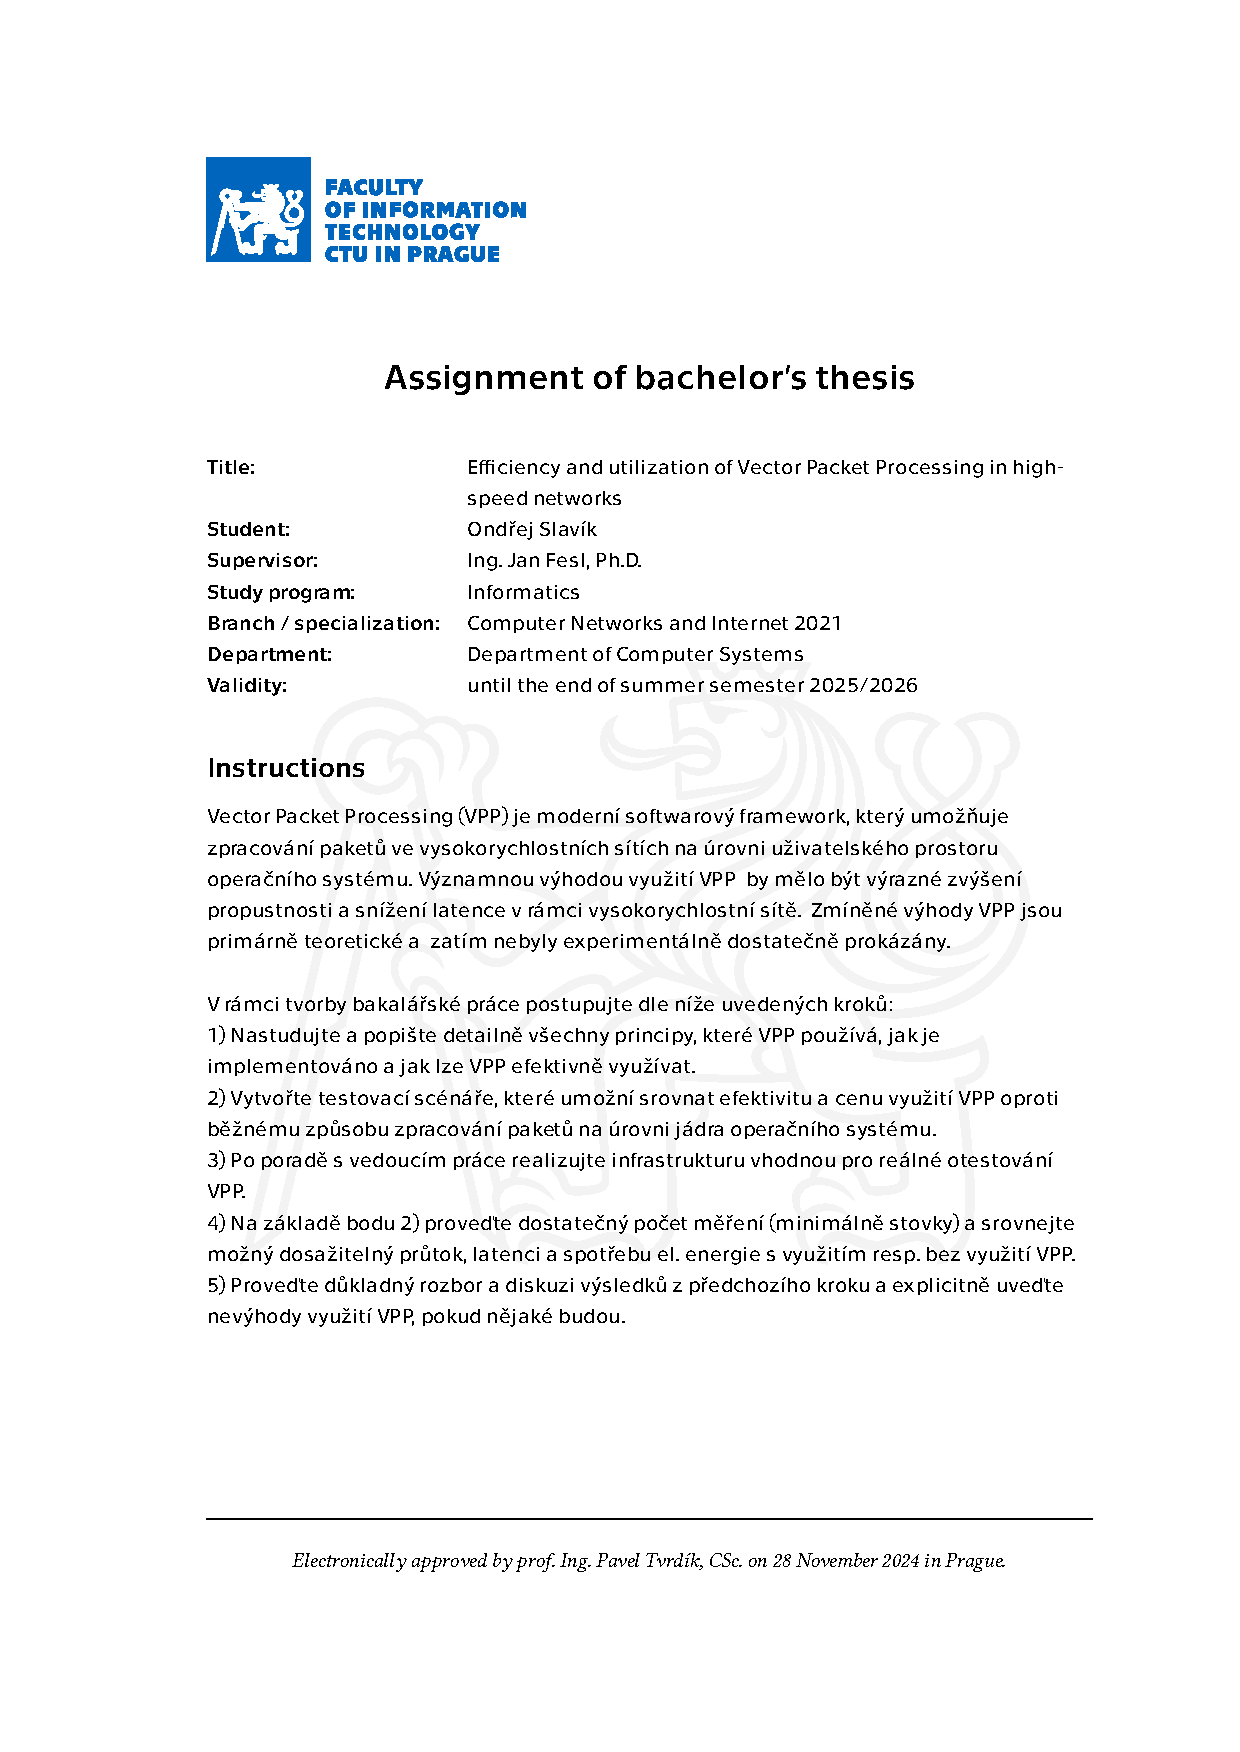
\includepdf[pages={1-}]{zadani.pdf} % replace this file with your thesis assignment generated from ProjectsFIT

\imprintpage % do not remove this command
\stopTOCentries
%%%%%%%%%%%%%%%%%%%%%%
% list of other contents END
%%%%%%%%%%%%%%%%%%%%%%

%%%%%%%%%%%%%%%%%%%
% ACKNOWLEDGMENT
% FILL IN / MODIFY
% This is a place to thank people for helping you. It is common to thank your supervisor.
%%%%%%%%%%%%%%%%%%%
\begin{acknowledgmentpage}
I would like to express my sincere gratitude to my thesis supervisor, Ing. Jan Fesl, Ph.D., for his guidance, support, and valuable insights throughout the entire process of writing this thesis.

My thanks also go to the Silicon Hill club of the CTU Student Union for providing an inspiring environment and the technical resources that supported my work.

Finally, I would like to thank my family for their unwavering support, encouragement, and never-ending patience during my studies.
\end{acknowledgmentpage} 
%%%%%%%%%%%%%%%%%%%
% ACKNOWLEDGMENT END
%%%%%%%%%%%%%%%%%%%


%%%%%%%%%%%%%%%%%%%
% DECLARATION
% FILL IN / MODIFY
%%%%%%%%%%%%%%%%%%%
% INSTRUCTIONS
% ENG: choose one of approved texts of the declaration. DO NOT CREATE YOUR OWN. Find the approved texts at https://courses.fit.cvut.cz/SFE/download/index.html#_documents (document Declaration for FT in English)
% CZE/SLO: Vyberte jedno z fakultou schvalenych prohlaseni. NEVKLADEJTE VLASTNI TEXT. Schvalena prohlaseni najdete zde: https://courses.fit.cvut.cz/SZZ/dokumenty/index.html#_dokumenty (prohlášení do ZP)
\begin{declarationpage}
I hereby declare that the presented thesis is my own work and that I have cited all sources of
information in accordance with the Guideline for adhering to ethical principles when elaborating an
academic final thesis.

I acknowledge that my thesis is subject to the rights and obligations stipulated by the Act No.
121/2000 Coll., the Copyright Act, as amended. In accordance with Section 2373(2) of Act No.
89/2012 Coll., the Civil Code, as amended, I hereby grant a non-exclusive authorization (licence) to
utilize this thesis, including all computer programs that are part of it or attached to it and all
documentation thereof (hereinafter collectively referred to as the "Work"), to any and all persons
who wish to use the Work. Such persons are entitled to use the Work in any manner that does not
diminish the value of the Work and for any purpose (including use for profit). This authorisation is
unlimited in time, territory and quantity.

I declare that I have used AI tools during the preparation and writing of my thesis. I have verified
the generated content. I confirm that I am aware that I am fully responsible for the content of the
thesis.
\end{declarationpage}
%%%%%%%%%%%%%%%%%%%
% DECLARATION END
%%%%%%%%%%%%%%%%%%%

\printabstractpage % do not remove this command

%%%%%%%%%%%%%%%%%%%
% SUMMARY
% FILL IN / MODIFY
% OR REMOVE ENTIRELY (upon agreement with your supervisor)
% (appropriate to remove in most theses)
%%%%%%%%%%%%%%%%%%%
% \begin{summarypage}
% \section*{Summary section}
% 
% \lipsum[1][1-8]
% 
% \section*{Summary section}
% 
% \lipsum[2][1-6]
% 
% \section*{Summary section}
% 
% \lipsum[3]
% 
% \section*{Summary section}
% 
% \lipsum[2]
% 
% \section*{Summary section}
% 
% \lipsum[1][1-8] Lorem lorem lorem.
% \end{summarypage}
%%%%%%%%%%%%%%%%%%%
% SUMMARY END
%%%%%%%%%%%%%%%%%%%

\tableofcontents % do not remove this command
%%%%%%%%%%%%%%%%%%%%%%
% list of other contents: figures, tables, code listings, algorithms, etc.
% add/remove commands accordingly
%%%%%%%%%%%%%%%%%%%%%%
\listoffigures % list of figures
\begingroup
\let\clearpage\relax
\listoftables % list of tables
\thectufitlistingscommand
\endgroup

%%%%%%%%%%%%%%%%%%%
% ABBREVIATIONS
% FILL IN / MODIFY
% OR REMOVE ENTIRELY
% List the abbreviations in lexicography order.
%%%%%%%%%%%%%%%%%%%
\chapter{\thectufitabbreviationlabel}
	
\begin{tabular}{rl}
API & Application Programming Interface\\
BIRD & BIRD Internet Routing Daemon\\
BPWh & Bytes Per Watt-Hour\\
CLI & Command-Line Interface\\
CNF & Cloud-Native Network Function\\
DMA & Direct Memory Access\\
DPDK & Data Plane Development Kit\\
DUT & Device Under Test\\
ECMP & Equal-Cost Multi-Path\\
FD.io & Fast Data Project\\
GRO & Generic Receive Offload\\
GRE & Generic Routing Encapsulation\\
GTP-U & GPRS Tunneling Protocol - User plane\\
IRQ & Interrupt Request\\
L2 & Layer 2 (Data Link Layer)\\
L3 & Layer 3 (Network Layer)\\
L4 & Layer 4 (Transport Layer)\\
Linux & Linux kernel network stack\\
MTU & Maximum Transmission Unit\\
NAT & Network Address Translation\\
NFV & Network Function Virtualization\\
NIC & Network Interface Card\\
NUMA & Non-Uniform Memory Access\\
PMD & Poll Mode Driver\\
PPWh & Packets Per Watt-Hour\\
RSS & Receive Side Scaling\\
SDN & Software Defined Networking\\
VLIB & Vector Library\\
VNET & Vector Network Layer\\
VNF & Virtual Network Function\\
VPP & Vector Packet Processing\\
VXLAN & Virtual Extensible LAN\\
\end{tabular}

%%%%%%%%%%%%%%%%%%%
% ABBREVIATIONS END
%%%%%%%%%%%%%%%%%%%
\resumeTOCentries
\mainmatter\mainmatterinit % do not remove these two commands
%%%%%%%%%%%%%%%%%%%
% THE THESIS
% MODIFY ANYTHING BELOW THIS LINE
%%%%%%%%%%%%%%%%%%%

% Do not forget to include Introduction
%---------------------------------------------------------------
%\chapter{Introduction}
% uncomment the following line to create an unnumbered chapter
\chapter*{Introduction}\addcontentsline{toc}{chapter}{Introduction}\markboth{Introduction}{Introduction}
%---------------------------------------------------------------
\setcounter{page}{1}

% The following environment can be used as a mini-introduction for a chapter. Use that any way it pleases you (or comment it out). It can contain, for instance, a summary of the chapter. Or, there can be a quotation.
%\begin{chapterabstract}
%\end{chapterabstract}

Modern high-performance network devices are usually proprietary systems that combine custom hardware, specialized operating systems, and tightly coupled software. 
While these solutions offer high throughput and reliability, they are typically expensive, inflexible, and slower to evolve due to their closed design and development model.
Vector Packet Processing (VPP) is a high-performance network stack that operates at layers 2 to 4 of the ISO/OSI model. 
It was originally developed by Cisco Systems, Inc. (which is a world leader in networking) and open-sourced in 2016 under the Fast Data Project (FD.io), that is part of the Linux Foundation.
VPP brings the ability to perform efficient, high-speed packet processing on common off-the-shelf (COTS) hardware, across a wide range of platforms and operating systems.
Its open and flexible architecture opens the door to a new class of network applications that can be deployed and scaled more easily than traditional hardware appliances. 
In this way, VPP could represent a shift in the traditionally conservative networking world, echoing the "Mainframe to PC" revolution, 
where general-purpose systems replaced proprietary platforms, enabling broader innovation and accessibility.

Since VPP was open-sourced only recently, it has not yet been widely adopted by the market, and there are only a limited number of academic studies on the subject. As a result, this area remains underexplored. 
This thesis aims to contribute to this field by evaluating VPP's\footnote{The abbreviation VPP is also commonly used in academic literature to refer to a Virtual Power Plant.} performance, 
with a particular focus on its electricity consumption. 
The findings could provide valuable insights for the industry and guide future research, especially in light of the increasing importance of energy efficiency, 
as highlighted in recent forecasts by ČEPS a.s. regarding the future of energy resources in the Czech Republic.

With the development of AI and the growing demand for high-resolution streaming services, it is highly likely that the demand for internet bandwidth will continue to rise. 
This will result in an increased need for network equipment capable of processing larger volumes of data more efficiently. 
Therefore, it is crucial to explore technologies like VPP that are capable to handle this growing demand and to explore their energy efficiency.

This thesis is divided into two parts: Theoretical and Practical. 
The Theoretical part presents the traditional approach to networking and packet processing, as well as an overview of how VPP is designed and the principles on which it operates. 
Additionally, it introduces the testing scenarios that were used. 
The Practical part describes the testing infrastructure, presents the results of various measurements, and provides an analysis of the findings.

%---------------------------------------------------------------
\chapter{Theoretical part}
%---------------------------------------------------------------

%---------------------------------------------------------------
\section{Vector Packet Processing (VPP) and Its Operating Principles}
%---------------------------------------------------------------
\begin{chapterabstract}
This section describes the fundamental principles behind the Vector Packet Processing (VPP) technology, which aims to enable efficient and high-performance network packet processing. 
VPP is built on modern programming and architectural principles that allow maximum utilization of contemporary hardware, particularly in parallel processing and memory access optimization.
\end{chapterabstract}

The section begins with a brief description of traditional network traffic processing methods used by operating systems and their limitations in terms of performance and scalability. 
Following that, the architecture of VPP is explored in detail, explaining how packets are processed in vectors, the use of a node graph, 
and the various techniques that contribute to its high efficiency—such as I/O and compute batching, zero-copy methods, and lock-free multi-threading. 
The purpose of this section is to provide a theoretical foundation for understanding how VPP operates.

\subsection{Traditional network traffic processing}
A \textit{network packet} is a basic unit of data transmitted over a network. It consists of a \textit{header}, which includes control information such as source and destination IP addresses, 
and a \textit{payload}, which carries the actual user data. 
Packets are routed independently through the network and reassembled at the destination. 
This structure allows efficient and reliable communication, even over complex or unreliable network paths.

Currently, packet processing works as follows: a packet arrives at the network card, which then
issues a system call (syscall) to the operating system for packet processing. The microprocessor
must save the currently executing instruction, perform a context switch, locate the appropriate
service routine in the interrupt vector table, and handle the packet processing. Once completed, it
must restore the saved instruction, perform another context switch, and return to processing the
interrupted program.

This system for operating peripherals was designed under the assumption that the peripherals
would not request interrupts continuously, which is not the case with network devices that need
to process large volumes of data split into small parts. 
This method requires the microprocessor to execute a significant
number of instructions not directly related to packet processing. 
Chase et al. \cite{gallatin1999trapeze} discovered \footnote{kap. 3.3 obr. 6} that if MTU is 1500 bytes, then interrupt handling accounts for 20\% - 25\% of receiver packet-processing overhead.
Another disadvantage of tradidtional packet processing is the inefficient handling of cache memory; the processing of the packets one by one in response to
interrupts leads to frequent cache misses in both cache \& inctruction caches.\footnote{kap. 4.2}\cite{cox2000profiling} 

%-----------------------------------------------------
\subsection{An Introduction to VPP}

Vector Packet Processing (VPP) is a multi-platform network stack that operates at layers 2-4 of the ISO/OSI model and is developed by the FD.io project. 
It consists of a set of forwarding vertices arranged in an oriented graph and auxiliary software and provides out-of-the-box switch/router functionality.
Unlike traditional network stacks, which run in the kernel, VPP operates in user space.

In a traditional approach, packets are processed one by one. In contrast, VPP reads the largest available number of packets called vector from the network interface card (NIC) 
and processes the entire vector through a VPP node-graph one node at a time. Each node in this graph handles a specific part of the packet processing.
This approach reduces cache misses and spreads fixed overhead costs across multiple packets, lowering the average processing cost per packet. 
Additionally, it allows VPP to take advantage of multiple cores, enabling parallel processing, which significantly improves overall performance.

Vector Packet Processing (VPP) runs on common off-the-shelf hardware (COTS), ensuring its broad compatibility and flexibility for deployment. 
It supports various architectures such as x86, ARM, and Power, and can be deployed on both standard servers and embedded devices. 
The design of VPP is agnostic to hardware, kernel, and deployment platform, meaning it can operate across a wide range of systems, including bare metal servers, virtual machines (VMs), and containers. 
This approach allows VPP to be deployed on widely available infrastructure without the need for specialized hardware.\cite{fdio_what_is_vpp}

\subsection{Techniques used in VPP}

TBD
DOPAST !!! Low-level code optimization technique

According to Linguaglossa et al.\cite{LINGUAGLOSSA} VPP uses theese kernel-bypass techniques:

\begin{itemize}
  \item \textbf{Lock-Free Multi-Threading (LFMT)}
is a programming technique that leverages modern multi-core CPUs to increase system performance. In network applications, parallelism is achieved by running multiple threads in the same time. 
Ideally, the more threads are used, the better the system performance but only up to a saturation point beyond which additional threads bring no gainns. 
However, to reach this ideal performance, traditional synchronization mechanisms such as mutexes and semaphores must be avoided, as they introduce delays due to thread contention. 
Instead, lock-free architectures have to be used, allowing threads to operate independently without blocking each other. 
In the context of VPP this approach is enabled by hardware features like multi-queue NICs, 
which allow each thread to handle a distinct subset of traffic, ensuring efficient and parallel processing.

  \item \textbf{I/O batching (IOB)}
is a key technique used in VPP. 
Instead of raising an interrupt for every incoming packet, the network interface card (NIC) collects multiple packets into a buffer and triggers an interrupt only when the buffer is full. 
This reduces the overhead caused by frequent context switching and interrupt handling. 
VPP typically uses poll-mode drivers, which collect packets in batches without relying on interrupts. 
Moreover, the batching technique is applied system-wide in VPP. This approach maximizes CPU efficiency, improves cache usage, and delivers stable, high-throughput performance even under heavy load.

  \item \textbf{Compute batching (CB)} 
is a technique that extends I/O batching to the processing phase itself. 
Instead of processing one packet at a time, network functions are designed to operate on entire batches of packets. 
This approach minimizes overhead from function calls (such as context switches and stack setup) and improves instruction cache efficiency. 
When a batch of packets enters a processing function, only the first packet might cause an instruction cache miss, while the rest benefit from already-warmed cache.
Additionally it is possible to take advatage of instruction-level parallelism.
  
  \item \textbf{Receive-Side Scaling (RSS)}
is a hardware-based technique used by modern NICs to distribute incoming packets across multiple RX queues. 
This enables parallel packet processing by allowing each queue to be handled by a separate thread, improving scalability and throughput. 
Packet assignment is typically done using a hash function over packet header fields (e.g., the 5-tuple). 

  \item \textbf{Zero-Copy (Z-C)} 
is a technique used to eliminate unnecessary memory copying during packet processing. 
Instead of copying incoming packets from the network interface card (NIC) to a separate buffer via system calls, 
the NIC writes packets directly into a pre-allocated memory region that is shared with the user-space application via Direct Memory Access (DMA). 
This allows the application to access packet data without invoking system calls or duplicating memory, significantly reducing CPU overhead. 

  \item \textbf {Cache Coherence and Locality (CC\&L)} are critical factors in the performance of modern software-based packet processing systems. 
In current COTS architectures, memory access has become a major bottleneck, which is mitigated by a multi-level cache hierarchy.
Minimizing cache misses and maintaining data locality during packet processing is essential for achieving high performance and low latency.

  \item \textbf {Low-Level Parallelism (LLP)} 
refers to the ability to exploit the internal micro-architecture of modern CPUs, including multi-stage pipelines, arithmetic-logical units (ALUs), and branch predictors that help maintain pipeline efficiency. 
Well-optimized code can keep these pipelines full and execute multiple instructions per clock cycle, increasing overall throughput. 
Performance can be further improved by giving hints to the compiler -- such as indicating the likely outcome of conditional branches -- to reduce pipeline stalls. 
Vectorized packet processing and specific coding practices can take full advantage of these hardware features and VPP was specifically designed to taky advantage of LLP.

\end{itemize}

\subsection{VPP Processing Graph and Graph nodes}
At the core of VPP (Vector Packet Processing) lies the Packet Processing Graph, a directed graph composed of relatively small, modular \& loosely coupled nodes. 
Each node is designed to perform a specific task and there are 3 types of them: \textit{process}, \textit{input} \& \textit{internal}. 
Process nodes do not participate in the packet forwarding graph; instead, they handle timers, events, and other background tasks within the VPP runtime.
Input nodes are used for input of data and internal nodes are used for vector processing. Internal nodes also serves as output nodes. 
When a vector of packets is prepared by input node, it is then pushed through the internal nodes. 
During processing, the vector may be split if the batch contains packets of different protocols or types, as they may need to follow different paths through the graph
When the original vector is completely processed, the process repeats.
Illustration of this Processing Graph is shown in fig. \ref{fig:processing-graph}.

\begin{figure}[!htbp]
    \centering
    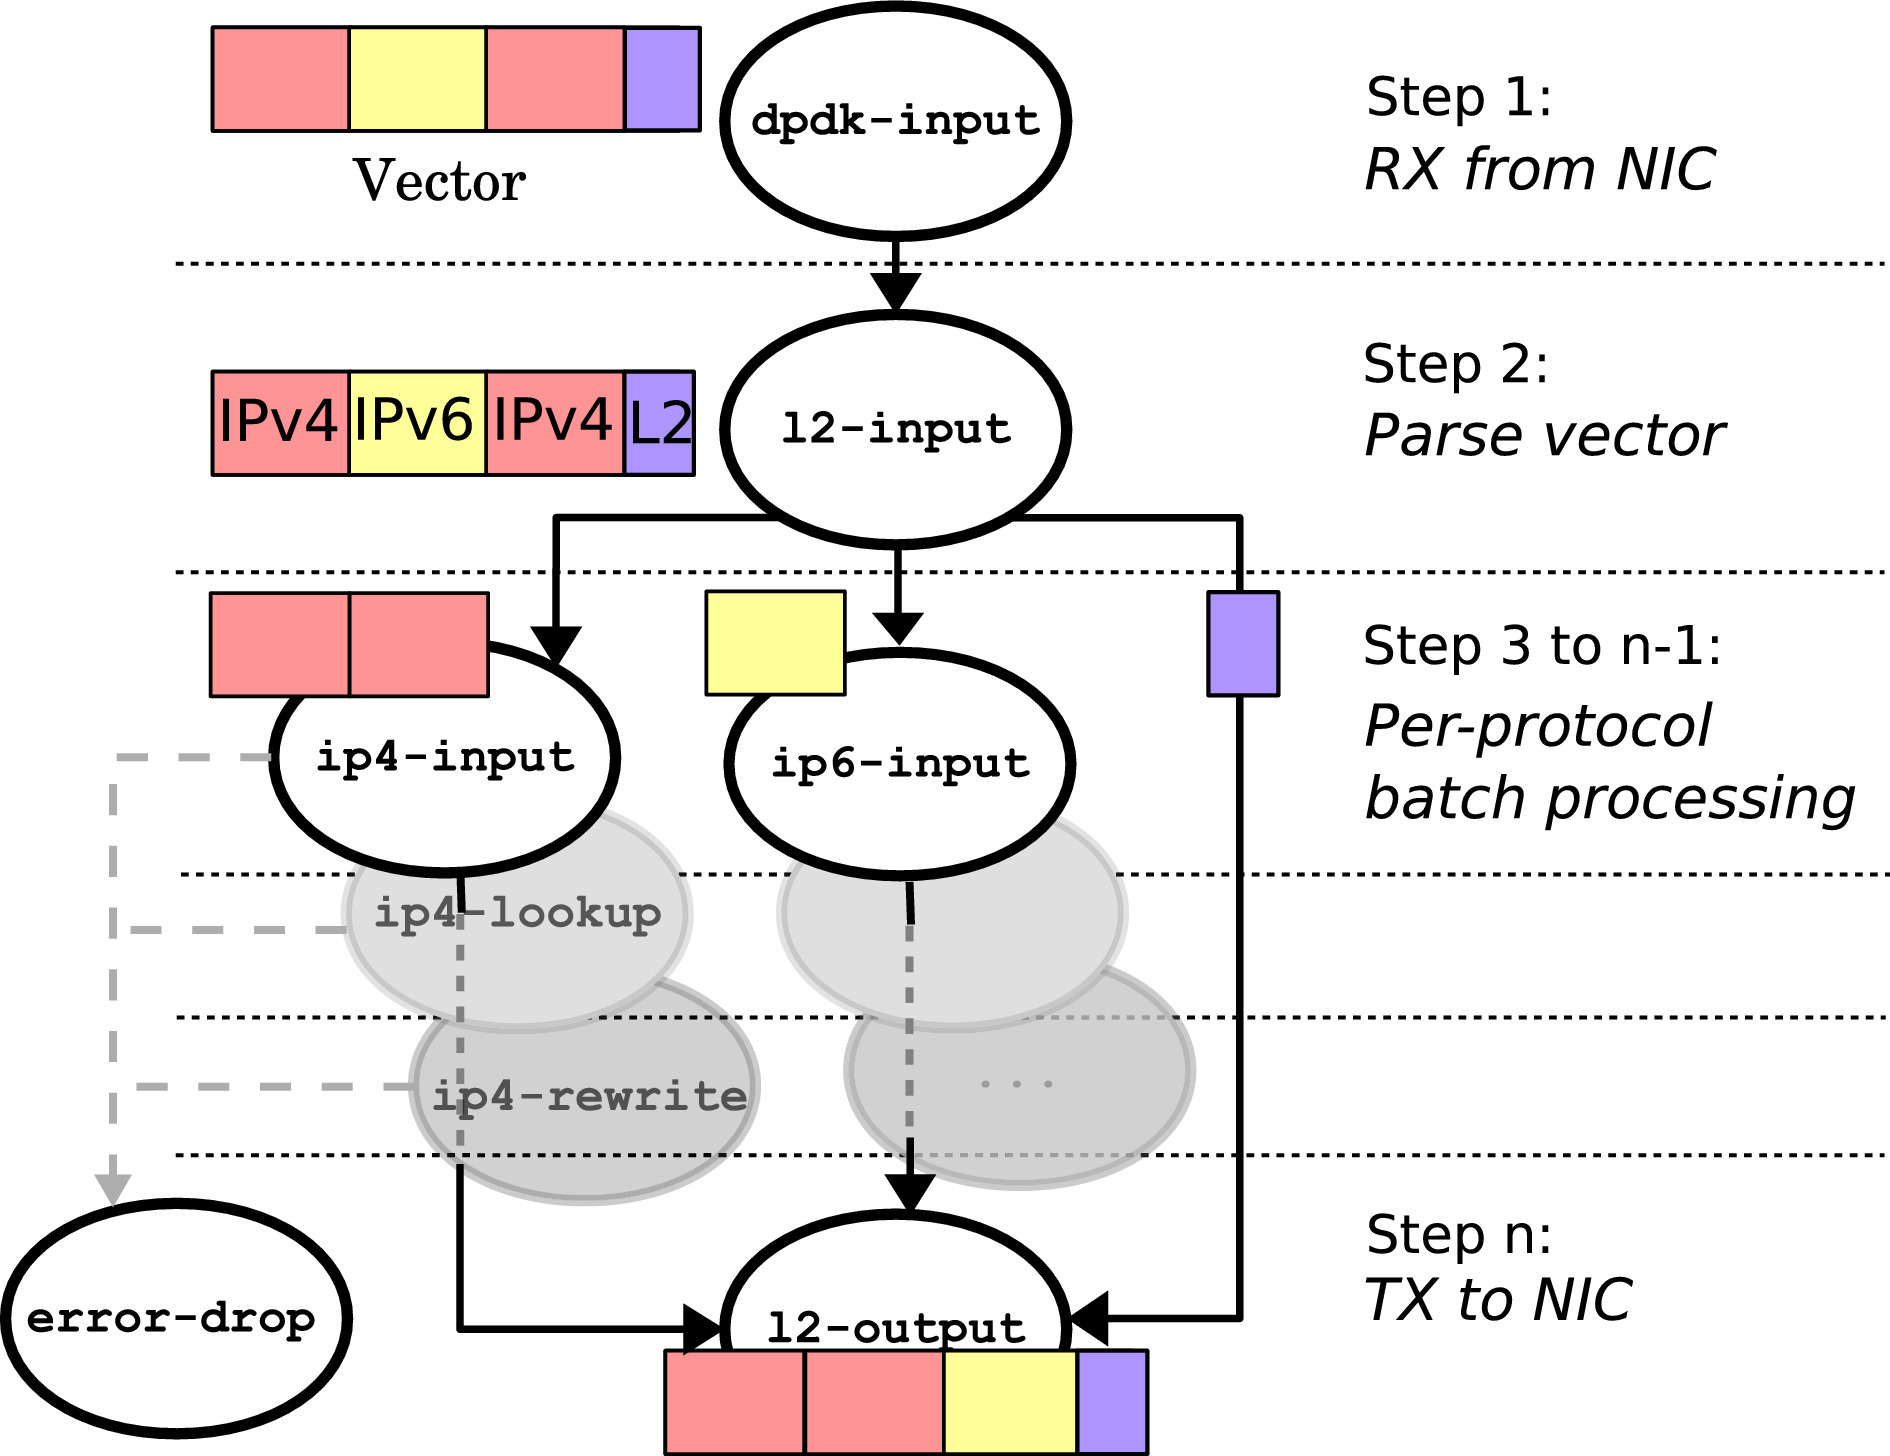
\includegraphics[width=0.7\linewidth]{images/processing-graph.jpg}
    \caption{Picture showing the VPP Processing Graph~\cite{LINGUAGLOSSA}}
    \label{fig:processing-graph}
\end{figure}

Thanks to VPP's modular design, the processing graph is highly customizable and extensible. 
New nodes -- referred to as plugins -- can be easily added to implement specific functionality or repleace existing ones. 
Plugins are shared libraries that are loaded during startup of VPP, and they are not dependent on the VPP source code, allowing them to be developed independently. 
Moreover, existing nodes can be rewired to modify the packet processing logic when necessary.\cite{LINGUAGLOSSA, DR:COMMAG-18, fdio_vpp_extensible_2021}

%--------------------------------------------------------------------
\subsection{DPDK and Its Role in VPP}
The Data Plane Development Kit (DPDK) is an open-source collection of libraries and drivers designed to support high-speed packet processing in user space. 
It was initially developed by Intel in 2010 and is now maintained as a Linux Foundation project. 
DPDK provides a set of APIs and components that allow applications to bypass the kernel network stack and directly access network interface cards (NICs) 
through poll-mode drivers (PMD), significantly reducing the overhead associated with traditional packet handling mechanisms.\cite{dpdk_about}

DPDK is used in VPP for interfacing with hardware. It is implemented as a plugin called \textit{dpdk-plugin}.\cite{LINGUAGLOSSA, DR:COMMAG-18} 

While VPP supports multiple mechanisms for accessing network devices, such as \textit{af\_packet}, to the best of the author's knowledge, DPDK is by far the most widely used option.

%--------------------------------------------------------------------
\subsubsection{Poll Mode Drivers}
Poll Mode Drivers (PMDs) are a key component of the DPDK framework. Unlike traditional network drivers, which rely on interrupts to signal packet arrival, 
PMDs continuously poll the network interface card (NIC) (specifically its RX queue) in a busy-loop, completely avoiding traditional interrupt-based mechanisms. 
This approach allows packets to be retrieved, processed, and delivered directly to user space without kernel involvement. 
While this results in very low latency and high throughput, it also causes constant CPU utilization on the cores assigned to polling, regardless of actual traffic load.\cite{FREITAS2022148}

Not every network interface card is supported by DPDK. Each supported device requires a specific Poll Mode Driver (PMD), which must be available and compatible with the given hardware. 
An up-to-date list of supported NICs and their corresponding PMDs is maintained on the official DPDK website.\cite{dpdk-supported-nics}

%--------------------------------------------------------------------
\subsubsection{Memory management and Hugepages}
DPDK uses a user-space memory model that eliminates the need for kernel involvement during packet processing. 
It operates on memory regions reserved as hugepages -- large memory pages, typically 2 MB or 1 GB in size, which are allocated at startup. 
These hugepages are used to store packet buffers and manage memory pools. 
DPDK defines its own memory management structures, such as mempools, which consist of preallocated fixed-size objects. 

DPDK is also explicitly NUMA-aware. Most memory allocation functions require the application to specify the target NUMA node, ensuring that memory is allocated close to the CPU core accessing it. 
This minimizes latency caused by cross-node memory access and helps optimize performance on multi-socket systems.\cite{burakov2019memory}

%--------------------------------------------------------------------
\subsubsection{Packet Reception and Transmission: A comparison between Linux Network Stack and DPDK}
When a packet arrives at a NIC managed by the Linux Network Stack, it is first stored in the NIC’s internal buffers. 
The NIC then writes the packet via Direct Memory Access (DMA) to the section of RAM provided by the driver and updates the corresponding descriptor in the RX buffer. 
The RX buffer is implemented as a ring queue.

Once the packet has been saved, the corresponding interrupt request (IRQ) is triggered to notify the CPU that one or more packets have arrived in that queue. 
Then, the corresponding IRQ handler is executed, which acknowledges the interrupt and calls the \textit{napi\_schedule} and \textit{\_\_raise\_softirq\_irqoff} functions.

The first function marks the associated \texttt{napi\_struct}%
\footnote{\texttt{napi\_struct} represents a NAPI context associated with a specific receive queue of a network device.}
 as ready for processing, while the second one raises a software interrupt (SoftIQR) specifically intended for processing incoming packets. 
Once the SoftIRQ is triggered, the kernel handles the actual packet processing in a deferred context. 
It goes through a list of network devices that have indicated pending work (i.e., their associated \texttt{napi\_struct} has been marked as ready) 
and calls their associated poll functions to retrieve and process packets from the receive queues.

This happens on the same CPU core that handled the original interrupt. If the system is busy or the processing takes too long, the remaining work may be handled by the \textit{ksoftirqd} kernel thread. 
The packets may be aggregated into a single larger packet using Generic Receive Offload (GRO), or processed individually. 
In both cases, they are passed to the IP stack via the \texttt{netif\_receive\_skb} function.

The transmission path is handled in a similar manner, using ring buffers, DMA, and deferred processing. 
However, unlike reception, packet transmission is initiated from the IP stack using the \texttt{\_\_dev\_queue\_xmit} function. 
Depending on the qdisc in use, packets are either enqueued in the software queue or passed directly to the driver for transmission.
Once a packet is selected for transmission, the driver places a descriptor into the TX ring buffer and sets up DMA so that the NIC can read the packet data from memory.
After the NIC finishes transmitting the packet, it triggers a TX interrupt, which allows the driver to perform post-processing such as unmapping DMA buffers and freeing memory.\cite{linux-packet-input}


When there is a NIC with multiple RX queues available, it is assigned to one of the queues based on the NIC's configuration%
\footnote{For network interface cards with multi-queue capabilities, the corresponding kernel driver often provides a module parameter to define how many hardware queues should be initialized and utilized.}.
The selection of the target queue is typically based on a hash function computed over network and/or transport layer headers.
Each queue has a dedicated IRQ, which can be assigned to specific CPU cores based on system settings. This mechanism is known as Receive Side Scaling (RSS).

When sending a packet from a NIC equipped with multiple TX queues, Transmit Packet Steering (XPS) is used to determine the appropriate TX queue.
The first option is that a CPU core is assigned specific TX queues. The second option is to use the TX queue corresponding to the RX queue from which the flow originated.
If multiple queues are eligible, a hash function is used to select the specific queue.\cite{linux-rss}

On the other hand, in DPDK the incoming packets are delivered by the network interface card (NIC) using direct memory access (DMA), 
which writes packet data into pre-allocated memory buffers specified by receive (Rx) descriptors.
These descriptors are organized in a circular ring (Rx queue), where the NIC populates entries at the head, while the VPP continuously polls the tail using functions such as                    
\textit{rte\_eth\_rx\_burst()}. This polling mechanism enables the VPP to retrieve multiple packets in a batch,
minimizing interrupt overhead and reducing latency, thereby increasing throughput and core efficiency.\cite{intel-core-utilization-2025}
 
Transmission is handled similarly, using a ring buffer known as the transmit (Tx) queue.
The application prepares transmit (Tx) descriptors at the tail of this queue, each containing the address and length of the packet to be sent.
These descriptors reference memory buffers (mbufs) holding the packet data. 
After the descriptors are written, the application updates the Tx queue’s tail pointer to notify the NIC that new packets are available.
The NIC then reads the descriptors from the head of the queue, fetches the packet data via DMA, and transmits the packets on the wire.\cite{intel-pcie-traffic-2025}

\begin{figure}[!htbp]
    \centering
    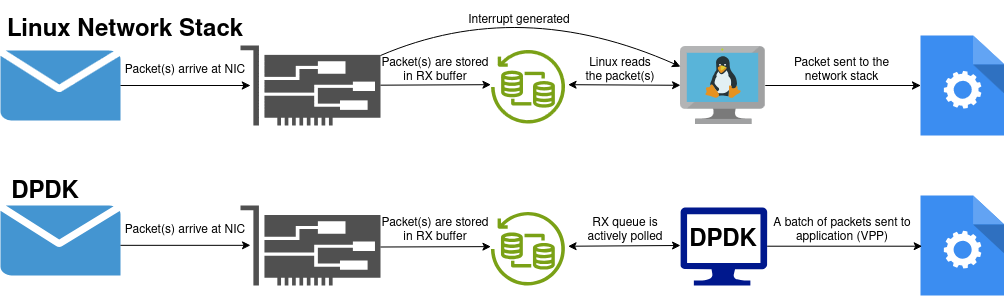
\includegraphics[width=0.99\linewidth]{images/dpdk-vs-linux.png}
    \caption{Diagram illustrating the differences in packet handling between the Linux Network Stack and DPDK.}
    \label{fig:dpdk}
\end{figure}

%COMPARISON
Based on the description above, several key differences between the Linux Network Stack and DPDK can be observed.
Although both rely on a similar underlying mechanism -- ring buffer queues -- their implementations differ fundamentally.
In the Linux Network Stack, memory management is handled by the kernel through device drivers. 
In contrast, DPDK allocates memory in user space and manages it through its own framework, providing packet buffers and ring structures directly to the application.

Linux is heavily dependent on hardware interrupts (IRQs) for packet reception and software interrupts (softIRQs) for deferred processing, which introduces frequent context switches. 
While NAPI uses polling to process packets from receive queues, they are still handled one at a time.
This increases the likelihood of cache misses during packet processing, as each packet is processed independently and may not benefit from cache locality.

In contrast, DPDK works entirely in user space and uses continuous active polling, completely bypassing the need for interrupts and context switching. 
Since it does not wait for an interrupt to occur, packet processing can begin sooner, reducing initial latency. 
Additionally, DPDK can retrieve multiple packets in a single burst, preparing them for vectorized processing in VPP.
Figure \ref{fig:dpdk} presents a simplified diagram highlighting the key differences.


%---------------------------------------------------------------
\section{Implementation of Vector Packet Processing}
%---------------------------------------------------------------
\subsection{DPDK and Its Role in VPP}

přesunout

The Data Plane Development Kit (DPDK) is an open-source collection of libraries and drivers designed to support high-speed packet processing in user space. 
It was initially developed by Intel in 2010 and is now maintained as a Linux Foundation project. 
DPDK provides a set of APIs and components that allow applications to bypass the kernel network stack and directly access network interface cards (NICs) 
through poll-mode drivers, significantly reducing the overhead associated with traditional packet handling mechanisms.\cite{dpdk_about}

The DPDK completely bypasses the kernel, communicating directly with the NIC.
DPDK avoids the use of the kernel’s system calls, instead handling its own I/O synchronization and memory management. 
DPDK employs a Poll Mode Driver (PMD) that uses busy-polling to retrieve, process, and deliver network packets to user-space applications without relying on interrupts. 
While this approach enhances performance by reducing latency, it also results in high CPU utilization, with the CPU usage on each core remaining close to 100\% regardless of the network load.\cite{FREITAS2022148}

DPDK is used in VPP for interfacing with hardware. It is implemented as a plugin called \textit{dpdk-plugin}.\cite{LINGUAGLOSSA, DR:COMMAG-18} 

%------------------------------------------
\subsection{VPP key architecture components}

VPP's dataplane is implemented by four main architectural layers: VPPINFRA, VNET, VLIB, and Plugins. 
Each layer provides distinct functionalities that support efficient networking operations, from low-level data structure management to high-level network function optimizations. 
The following sections describe these layers in detail: \footnote{https://my-vpp-docs.readthedocs.io/en/vpp-config/gettingstarted/developers/swarch/softwarearchitecture.html}

\begin{itemize}
  \item \textbf{VPPINFRA} -- layer providing foundational libraries for performing tasks with memory, vectors, rings, lookups in hash tables \& timers.
  \item \textbf{VNET} -- layer that deals with networking on layers 2 - 4 and is responsible for Control plane.
  \item \textbf{VLIB} -- layer that provides library for vector processing, implements CLI and handles application management functions.
  \item \textbf{Plugins} -- layer which is a set of plugins that allow for adding network functions and optimizations tailored to specific needs.
\end{itemize}

\subsubsection{VPPINFRA}
VPPINFRA is a collection of library services designed to offer high-performance capabilities for various tasks. 
It includes features such as dynamic arrays, hashes, bitmaps, high-precision real-time clock support, event logging, and data structure serialization. The following functionalities are implemented:

\begin{itemize}
  \item \textbf{Vectors} -- dynamically resized arrays with \textit{headers} defined by user. They serve as a core building block for other data structures (e.g., hash tables, pools) and allow efficient memory reuse via safe length resetting.
  \item \textbf{Bitmaps} -- dynamic bitmaps based on VPPINFRA vectors.
  \item \textbf{Pools} -- structures used to quickly allocate \& free fixed-size data structures. 
  \item \textbf{Hashes} -- structures thats provide fast key-value lookups, commonly mapping keys to indices in vectors or pools. Bihash is used in the data plane for fixed-size keys and is thread-safe, while the simpler hash is used in the control plane for exact string matching.
  \item \textbf{Timekeeping} -- service providing high-precision, low-cost timing based on CPU ticks. Since CPU ticks are not perfectly accurate, the system continuously adjusts its estimate of "ticks per second" by comparing with the kernel’s time. This results in precise and smooth time measurements without the need for expensive system calls. 
  \item \textbf{Timer wheel} -- system for efficiently managing timers or timeouts. It allows the user to define parameters like the number of wheels, slots per ring, and timers per object, optimizing time-based operations in systems requiring high-performance event management.
\end{itemize}

\subsubsection{VNET}
odmítám dělat teď

\subsubsection{VLIB}
Zítra je taky den

\subsubsection{Plugins}
Plugins are used to modify or create new features into the VPP. 
Developers can create plugins through a straightforward process, involving the generation of necessary files and integration into the build system. 
After building, the new plugin can be loaded and tested within the VPP environment. 

VLIB supports a simple mechanism for loading and using plugins. 
VLIB client applications specify a directory where the plug-ins are located and can apply a filter to narrow down the search. 
Once the plug-ins are loaded, VLIB ensures they are correctly registered and ready for use.


%--------------------------------------
\subsection{Configuration and Startup}


%---------------------------------------------------------------
\section{Utilization of Vector Packet Processing}
%---------------------------------------------------------------
VPP supports a comprehensive set of Layer 2 to Layer 4 network functions. 
At Layer 2, it provides Ethernet bridging, MAC learning, VLAN tagging (including dot1q and QinQ), and support for L2 cross-connects and policers.

At Layer 3, VPP implements both IPv4 and IPv6 routing with ECMP support, NAT44/NAT64, and ACL-based filtering. 
It also supports tunneling mechanisms such as GTP-U, IP-in-IP, and VXLAN. Segment routing (SRv6), LISP, and punt redirect mechanisms are included as well.

At the transport layer (L4), basic UDP and TCP stack functionality is available. 

Additionally, supported features include PPPoE, the WireGuard VPN protocol, GRE tunneling, DHCP client and proxy functionality, and L2TPv3.~\cite{fdio-vpp-features-2502}

According to the VPP's authors~\cite{fdio_what_is_vpp}, VPP can be for example effectively utilized as a virtual switch, virtual router, gateway or used as a basis for a firewall, IDS and load balancer.
It already includes enough features to be deployed in production environments.


\subsection{Integration with the SDN/NFV Ecosystem}
To meet the requirements of modern virtualized and cloud-native networking environments, Vector Packet Processing was architected with a clear separation between the data plane and control plane. 
This design choice enables its integration into SDN and NFV frameworks, where packet forwarding logic can operate independently from centralized control mechanisms. 
VPP's modularity and userspace implementation allow it to function efficiently within dynamic, multi-tenant infrastructure, 
while remaining compatible with orchestration systems and control-plane protocols commonly used in such deployments

VPP is fully compatible with both Virtual Network Functions (VNFs) and Cloud-Native Network Functions (CNFs). 
Its modular architecture allows deployment in environments utilizing service function chaining, Kubernetes-based orchestration, or OpenStack-based infrastructures. 
Because of its userspace design and performance-optimized data plane, VPP can serve as the fast packet processing backend for SDN-controlled systems and NFV orchestrators.~\cite{fdio2017whitepaper}

\subsection{VPP as a Complete Router Solution}
VPP is implemented solely as a data-plane, meaning it is not a complete routing solution on its own. 
VPP is dedicated to efficiently forwarding packets between interfaces based on routing rules and access control filters, 
but it does not include a native control-plane or support for dynamic routing protocols such as BGP or OSPF.

However, as demonstrated by the authors of the VBSR (VPP-Bird Software Router) project~\cite{10819057}, 
it is possible to integrate VPP with additional components such as the Linux Control Plane (Linux-CP) plugin and the BIRD routing daemon. 
Bird acting as a control-plane enables dynamic routing using protocols like BGP 
and the Linux-CP is responsible for communication between VPP and BIRD. 
This integrated system creates a nearly feature-complete router solution, comparable in functionality to commercial routers.

It is important to note, however, that firewall functionality is still limited and was left by authors of VBSR as a future work.~\cite{10819057} 
While VPP supports basic packet filtering through ACLs, it lacks advanced stateful firewall features~\cite{fdio-vpp-features-2502}. These would need to be handled externally.



%---------------------------------------------------------------
\section{Survey of Traffic Generation Tools}
%---------------------------------------------------------------
In order to evaluate the performance of network devices and data-plane frameworks such as VPP, synthetic traffic must be generated in a controlled and reproducible manner. 
Selecting appropriate traffic generation tools is therefore essential for conducting accurate benchmarking and stress-testing. Although numerous traffic generation tools exist~\cite{traffic-generators}, 
this section focuses on a subset commonly used for high-performance benchmarking and synthetic traffic generation in research and practice, namely iPerf3, D-ITG, TRex, Pktgen-DPDK \& Genesids. 

\begin{itemize}
  \item \textbf{iPerf3} -- iPerf3 is a network testing tool used to measure TCP, UDP, and SCTP throughput between two endpoints. It allows detailed configuration of testing parameters such as buffer size, number of parallel streams, test duration, and jitter. iPerf3 can also measure jitter, providing insights into the variation in packet arrival times, which is useful for evaluating network stability. Its client-server architecture makes it a common tool for performance benchmarking of networks and devices.~\cite{iperf}

  \item \textbf{D-ITG} -- Distributed Internet Traffic Generator is a network traffic generator designed to produce traffic flows that accurately emulate a wide range of real-world application behaviors. It supports multiple transport layer protocols, including TCP, UDP, DCCP, and SCTP. D-ITG allows users to define parameters such as packet size, inter-departure time, and number of flows, making it suitable for controlled experiments on delay, jitter, packet loss, and throughput. It can operate in both single-node and distributed modes, enabling flexible deployment for testing complex topologies and performance conditions. D-ITG also includes tools for logging and analyzing the generated traffic, facilitating detailed post-experiment evaluation.~\cite{DITGManual}

  \item \textbf{TRex} -- TRex, developed by Cisco, is a high-performance, stateful and stateless traffic generator built on top of DPDK. It supports the generation of realistic Layer 4–7 traffic using pre-recorded PCAP files and emulates multiple concurrent users and flows. TRex is especially suited for benchmarking network function virtualization (NFV) platforms, routers, and firewalls in both laboratory and production-like environments.~\cite{trex} 

\item \textbf{Pktgen-DPDK} -- Pktgen-DPDK is a high-performance traffic generator tool developed as part of the Data Plane Development Kit (DPDK). Pktgen-DPDK supports various network protocols, including IPv4, IPv6, UDP, and TCP. The tool allows precise control over traffic parameters, such as packet rate, size, and timing. Pktgen-DPDK is used in network performance tests and can capture packet-level statistics to assess the performance of the devices under test.~\cite{pktgen_dpdk} 
\end{itemize}

Among the reviewed tools, the author decided to utilize iPerf3 and TRex in the subsequent experimental evaluation. 
IPerf3 was selected due to its status as a de facto standard for basic throughput and jitter measurements, ease of use, and widespread adoption in academic and practical contexts. 
TRex was chosen for its modern architecture, support for high-speed stateful and stateless traffic generation, and ability to simulate real-world traffic. 
In addition, TRex provides a Python-based API that enables scripting and automation of test scenarios, making it well-suited for integration into continuous testing pipelines and reproducible experiments. 
Other tools, such as Pktgen-DPDK and D-ITG, were excluded due to their relatively complex usage (Pktgen-DPDK) or limited maintenance and outdated design (D-ITG).



%---------------------------------------------------------------
\chapter{Pratical part}
%---------------------------------------------------------------

%---------------------------------------------------------------
\section{Building Infrastructure for Measurement}
%---------------------------------------------------------------
The testing infrastructure has been implemented as recomended in RFC 2544~\cite{rfc2544}, which defines methods for evaluating network performance. 
It consists of a device under test (DUT), connected to a measurement device called Tester\footnote{The hardware used in this testing setup was loaned free of charge for the purposes of this bachelor thesis by Silicon Hill club.}.

The Device Under Test (DUT) and the measurement device are connected using 100~Gbit capable cables, preventing any potential bottlenecks in the connection.
The illustration of this hardware setup is shown in Fig. \ref{fig:hardware-setup}

\begin{figure}[!htbp]
    \centering
    
\includegraphics[width=0.9\linewidth]{images/setup.png}
    \caption{Picture showing hardware setup}
    \label{fig:hardware-setup}
\end{figure}

The Device Under Test (DUT) is the network device being evaluated during testing. 
It is configured with a specific network stack and settings based on measurement scenario.
The DUT is responsible for processing network traffic and responding to the test conditions set by the measurement device.
Additionally, the electrical power consumption of the DUT is monitored and measured during the tests to assess its energy efficiency under varying loads.
The hardware of DUT is shown in Table \ref{tab:hardware_dut}.

The Tester (Measurement Device), on the other hand, is responsible in generating the network traffic and capturing the responses from the DUT.
Its physical features are shown in Table \ref{tab:hardware_tester}. 

\begin{table}[h!]
\centering
\caption{Hardware details for DUT (Device Under Test)}
\begin{tabular}{|c|c|}
\hline
\textbf{Hardware Component} & \textbf{DUT (Device Under Test)} \\
\hline
\textbf{CPU Model} & 2x Intel(R) Xeon(R) CPU E5-2660 v3 \\
\hline
\textbf{Frequency} & 2.60GHz \\
\hline
\textbf{Cores} & 10 physical cores each (1 thread/core) \\
\hline
\textbf{Memory (RAM)} & 256 GB of DDR4 ECC \\
\hline
\textbf{NIC} & Mellanox ConnectX-6 Dx (Dual-port) \\
\hline
\end{tabular}
\label{tab:hardware_dut}
\end{table}


\begin{table}[h!]
\centering
\caption{Hardware details for Tester (Measurement Device)}
\begin{tabular}{|c|c|}
\hline
\textbf{Hardware Component} & \textbf{Tester (Measurement Device)} \\
\hline
\textbf{CPU Model} & 2x Intel(R) Xeon(R) Gold 6136 CPU \\
\hline
\textbf{Frequency} & 3.00GHz \\
\hline
\textbf{Cores} & 12 physical cores each (2 threads/core)\\
\hline
\textbf{Memory (RAM)} & 384 GB DDR4 ECC\\
\hline
\textbf{NIC} & 2x Mellanox ConnectX-5 \\
\hline
\end{tabular}
\label{tab:hardware_tester}
\end{table}

The DUT is running Debian GNU/Linux 12 (Bookworm) x86\_64 with Linux kernel version \textit{6.1.0-32-amd64}, VPP v25.02-release, and DPDK version 24.11.1. 
This kernel version is the current standard long-term support (LTS) release provided with Debian 12 (Bookworm) and was used for all tests involving the Linux networking stack.
The tester generates traffic using Cisco TRex version 3.06.


%---------------------------------------------------------------
\section{Metodology}
%---------------------------------------------------------------
The RFC 2544 recommends that each test be at least 60 seconds in duration~\cite{rfc2544}. 
In this work, the duration was extended to 120 seconds and each test was repeated 20 times to ensure greater stability and statistical relevance of the results. 
The reported values represent the arithmetic mean of these 20 measurements.
In cases where an error, anomalous spike or irregularity was observed in the results, the corresponding measurement was discarded and the test was repeated. 
All these steps were taken to ensure consistency and statistical reliability.

The following metrics were collected: the number of transmitted and received packets and bytes; average, minimum, and maximum one-way latency; jitter; 
and total energy consumption of the DUT, expressed in watt-hours.

All numerical results are rounded to two decimal places.
Since traffic generation was performed using TRex, its potential measurement inaccuracy must be taken into account when interpreting the results.
It should also be noted that in cases where packet loss occurred, higher deviations in delay and jitter statistics can be expected, as packet loss may negatively impact the consistency of these measurements.
To evaluate energy efficiency, the number of packets per watt-hour (PPWh) and bytes per watt-hour (BPWh) was used, considering only successfully delivered packets.
Power consumption was measured using a Raritan PX3-5498-K1 unit running firmware version 4.2.0.5-50274.
The idle power consumption of the DUT is approximately 5 Wh per two minutes.


%---------------------------------------------------------------
\section{Test Scenarios \& Results}
%---------------------------------------------------------------
TBD
%-------------------------------------------------------------------------------
\subsection{Bidirectional UDP 1 Gbit/s}
This section presents a set of performance and efficiency tests performed on the Device Under Test (DUT) using bidirectional UDP traffic at a total rate of 1\,Gbit/s. 
The goal is to evaluate the forwarding performance of the DUT under varying packet sizes, simulating realistic traffic patterns with increasing stress on the packet-processing path.

To provide a comprehensive and representative view, the tests are structured into five subsections, each corresponding to a different Ethernet frame size. 
Four of the selected sizes -- 64 bytes, 512 bytes, 1280 bytes, and 1518 bytes -- are recommended by RFC2544\cite{rfc2544} 
covering both edge-cases and practically relevant intermediate values. 
The fifth size, 889 bytes, was chosen because it was identified as the average size in real-world network traffic by Jurkiewicz et al.~\cite{JURKIEWICZ202115}. 
This selection covers the full range of standard Ethernet frame sizes, from the minimum to the maximum non-jumbo frames, 
and includes a representative average frame size observed in real network traffic.

Traffic in all scenarios is generated using TRex with the \textit{udp\_1pkt\_src\_ip\_split.py} profile, 
which ensures that each packet carries a unique source IP address to simulate multiple concurrent clients, while maintaining a single destination IP per direction. 
The routing table of the DUT contains only two active forwarding entries, corresponding to the test routes, in addition to two administrative entries used for management.
The total offered load is 1\,Gbit/s, symmetrically split between both directions (500\,Mbit/s each).
The chosen load of 1 Gbit/s is representative of a realistic aggregate traffic pattern that could be observed in a small or medium-sized enterprise network, especially when routed through a central gateway.

The DUT is configured with the Vector Packet Processing (VPP) stack and tested under three levels of parallelism: using 1, 4, and 10 worker threads. 
The number of RX/TX queues is aligned with the number of active worker threads in each configuration to ensure balanced packet distribution and optimal resource utilization.

To provide a baseline for comparison, all scenarios are also executed using the standard Linux kernel networking stack, 
configured with equivalent routing and interface parameters, but able to use all 20 cores of CPU. 
This allows for a direct comparison between VPP and traditional kernel-based forwarding in terms of performance and energy efficiency.

The aim of this test is to observe the behavior of the VPP forwarding plane under low traffic load of small packets and to evaluate its energy efficiency.

%-------------------------------------------------------------------------------
\subsubsection{64-bytes frames}
This test evaluates the behavior of the VPP forwarding plane under a low-throughput traffic load composed of minimum-sized Ethernet frames (64 bytes). 
Such frames result in a high packet-per-second rate for a given bandwidth, which increases the processing overhead per bit of data. 
This configuration represents a stress scenario for packet forwarding and allows assessment of the system’s efficiency in handling a large number of small packets.

\begin{table}[h!]
\centering
\begin{tabular}{|l|r|r|r|}
\hline
\multicolumn{1}{|c|}{\textbf{Configuration}} &
\multicolumn{1}{c|}{\textbf{Watts used}} &
\multicolumn{1}{c|}{\textbf{PPW}} &
\multicolumn{1}{c|}{\textbf{BPW}} \\
\hline
VPP -- 1 worker & 848.08 & 20 726 965.60 & 1 326 525 798.50 \\
VPP -- 4 workers & 951.03 & 18 483 249.76 & 1 182 927 982.40 \\
VPP -- 10 workers & 1 193.56 & 14 727 474.94 & 942 558 396.09 \\
Linux stack & 1 257.25 & 13 981 407.81 & 894 810 100.29 \\
\hline
\end{tabular}
\caption{Result of Bidirectional UDP 1 Gbit/s of 64-bytes packets test}
\label{tab:udp:one}
\end{table}

As the results in Table \ref{tab:udp:one} show, the power consumption increases notably with the number of worker threads in the VPP stack. 
While all VPP configurations deliver identical packet and byte throughput, the most energy-efficient setup in this measurement is the single-worker variant, consuming roughly 850 Watts during the test. 
In contrast, the traditional Linux network stack demonstrates the highest energy usage, despite handling the same volume of packets.

This discrepancy can likely be attributed to the cost of processing a high number of small packets in kernel space. 
Since the test uses fixed-size 64-byte frames, which are known to generate frequent system calls and context switches in Linux, 
the forwarding path becomes less efficient compared to VPP’s user-space architecture, where such overheads are significantly reduced. 
The results highlight the energy cost of kernel-based packet forwarding in scenarios dominated by small-packet traffic.

%------------------------------------------------------------------------------
\subsubsection{512-bytes frames}
This test focuses on the forwarding performance of the VPP data plane when processing medium-sized Ethernet frames of 512 bytes. 
These frames offer a balance between protocol overhead and payload efficiency and are representative of many real-world applications that do not utilize maximum frame sizes. 
The test helps to evaluate how the system handles typical traffic patterns with moderate packet rates and processing demands.

Notably, the 554-byte frame size (512 bytes of data) represents the historical maximum size of a DNS response over UDP without the use of extension mechanisms such as EDNS(0).\cite{satrapa2023dns} 

\begin{table}[h!]
\centering
\begin{tabular}{|l|r|r|r|}
\hline
\multicolumn{1}{|c|}{\textbf{Configuration}} &
\multicolumn{1}{c|}{\textbf{Watts used}} &
\multicolumn{1}{c|}{\textbf{PPW}} &
\multicolumn{1}{c|}{\textbf{BPW}} \\
\hline
VPP -- 1 worker & 851.21 & 2 581 343.78 & 1 321 648 015.98 \\
VPP -- 4 workers & 969.49 & 2 266 413.93 & 1 160 403 931.63 \\
VPP -- 10 workers & 1 175.07 & 1 869 901.91 & 957 389 779.06 \\
Linux stack & 965.58 & 2 275 591.60 & 1 165 102 847.70 \\
\hline
\end{tabular}
\caption{Result of Bidirectional UDP 1 Gbit/s of 512-bytes frames test}
\label{tab:udp:two}
\end{table}

As seen in the result Table \ref{tab:udp:two}, the power consumption of VPP remains stable. 
On the other hand, compared to the 64-byte scenario, the Linux stack shows improved energy efficiency when handling 512-byte packets. 
This is primarily due to the lower packet-per-second (PPS) rate associated with larger frames, which reduces the overhead caused by frequent context switches and system calls in the kernel space. 
Although the Linux stack remains slightly less efficient than VPP with one worker in this scenario, the margin is smaller than in the minimum-packet-size test.

%------------------------------------------------------------------------------
\subsubsection{889-bytes frames}
This test focuses on the forwarding performance of the VPP data plane when processing medium-sized Ethernet frames of 889 bytes. 
These frames offer a favorable balance between protocol overhead and payload efficiency. 
As mentioned earlier, this size was identified as the average frame size observed in real-world network traffic, according to a study by Jurkiewicz et al.~\cite{JURKIEWICZ202115}.

The test helps evaluate how the system handles traffic patterns that more closely resemble typical production environments, where packet sizes vary but tend to concentrate around this average. 
Compared to minimum-sized or maximum-sized frames, the 889-byte frame represents a realistic mid-point for both packet rate and processing complexity.

\begin{table}[h!]
\centering
\begin{tabular}{|l|r|r|r|}
\hline
\multicolumn{1}{|c|}{\textbf{Configuration}} &
\multicolumn{1}{c|}{\textbf{Watts used}} &
\multicolumn{1}{c|}{\textbf{PPW}} &
\multicolumn{1}{c|}{\textbf{BPW}} \\
\hline
VPP -- 1 worker & 853.27 & 1 483 079.03 & 1 318 457 253.58 \\
VPP -- 4 workers & 952.46 & 1 328 629.91 & 1 181 151 986.18 \\
VPP -- 10 workers & 1 190.42 & 1 063 042.32 & 945 044 623.54 \\
Linux stack & 940.33 & 1 345 768.87 & 1 196 388 523.99 \\
\hline
\end{tabular}
\caption{Result of Bidirectional UDP 1 Gbit/s of 889-bytes frames test}
\label{tab:udp:three}
\end{table}

As shown in Table \ref{tab:udp:three}, the third test with 889-byte frames, 
VPP's power consumption remains stable across different worker thread configurations. 
In the case of the Linux stack, energy efficiency improves slightly compared to the previous (512-byte) test, though the difference is minimal. 
The change is significantly smaller than the improvement observed between the 64-byte and 512-byte scenarios, suggesting that the impact of increasing frame size becomes less pronounced beyond a certain point.

%-------------------------------------------------------------------------------
\subsubsection{1280-bytes frames}
This test focuses on the forwarding performance of the VPP data plane when processing large Ethernet frames of 1280 bytes. 
These frames represent a size commonly used in environments where larger payloads are transferred, but without exceeding the typical Ethernet MTU limit of 1500 bytes. 
This size strikes a balance between higher data throughput and maintaining efficient protocol overhead.

The test evaluates how the system handles traffic patterns with higher packet sizes, which are common in applications involving large data transfers such as video streaming, 
file sharing, or other high-bandwidth scenarios in enterprise and data center environments.

\begin{table}[h!]
\centering
\begin{tabular}{|l|r|r|r|}
\hline
\multicolumn{1}{|c|}{\textbf{Configuration}} &
\multicolumn{1}{c|}{\textbf{Watts used}} &
\multicolumn{1}{c|}{\textbf{PPW}} &
\multicolumn{1}{c|}{\textbf{BPW}} \\
\hline
VPP -- 1 worker & 866.91 & 1 013 837.98 & 1 297 712 609.61 \\
VPP -- 4 workers & 961.01 & 914 565.18 & 1 170 643 425.56 \\
VPP -- 10 workers & 1188.39 & 739 577.31 & 946 658 957.41 \\
Linux stack & 926.77 & 948 354.26 & 1 213 893 456.20 \\
\hline
\end{tabular}
\caption{Result of Bidirectional UDP 1 Gbit/s of 1280-frames test}
\label{tab:udp:four}
\end{table}

The results in Table \ref{tab:udp:four} show a continued trend: power consumption increases with the number of worker threads, while throughput remains consistent across all VPP configurations. 
As in previous tests, the single-threaded setup achieves the best energy efficiency.

The Linux stack demonstrates slightly better energy efficiency than in the 889-byte test, but the improvement is again minimal. 
Compared to the large gain seen between the 64-byte and 512-byte cases, the impact of increasing frame size beyond this point becomes progressively less significant. 
This suggests diminishing returns in energy efficiency as packet sizes grow and per-packet processing overhead decreases.

%-------------------------------------------------------------------------------
\subsubsection{1518-bytes frames}
This test evaluates the performance of the VPP forwarding plane when handling full-sized Ethernet frames (1518 bytes, including headers). 
These frames represent the upper limit of standard Ethernet without jumbo frame extensions and provide throughput efficiency under optimal conditions, 
as the ratio of payload to protocol overhead is maximized. The goal is to observe how the system behaves when forwarding large packets that minimize per-packet processing overhead.

\begin{table}[h!]
\centering
\begin{tabular}{|l|r|r|r|}
\hline
\multicolumn{1}{|c|}{\textbf{Configuration}} &
\multicolumn{1}{c|}{\textbf{Watts used}} &
\multicolumn{1}{c|}{\textbf{PPW}} &
\multicolumn{1}{c|}{\textbf{BPW}} \\
\hline
VPP -- 1 worker & 854.66 & 867 136.33 & 1 316 312 956.40 \\
VPP -- 4 workers & 972.93 & 761 726.68 & 1 156 301 102.16 \\
VPP -- 10 workers & 1 192.34 & 621 556.55 & 943 522 846.94 \\
Linux stack & 930.32 & 796 614.86 & 1 209 261 363.10 \\
\hline
\end{tabular}
\caption{Result of Bidirectional UDP 1 Gbit/s of 1518-frames test}
\label{tab:udp:five}
\end{table}

As shown in Table \ref{tab:udp:five}, all VPP configurations deliver comparable throughput, with energy efficiency peaking once again in the single-threaded setup. 
Interestingly, the total power consumption of the VPP stack remains close to that observed in the other tests.

The Linux stack turned out to be slightly more power-hungry than in the previous test. 
However, the difference is small enough that it could fall within the margin of measurement error, suggesting that any further efficiency improvements with larger frames are likely negligible.

\subsubsection{Test Conclusion}
The VPP stack showed consistent power consumption across all tested frame sizes and thread configurations. 
This was expected, as VPP operates in a polling mode rather than being event-driven -- even when no packets are being processed, 
it continuously polls the network interface, keeping the CPU cores active regardless of traffic load or packet size.

The Linux stack, on the other hand, did not manage to outperform single-threaded VPP even in the most favorable condition -- when forwarding full-sized 1518-byte frames. 
This result highlights the inefficiency of the kernel-based packet processing path, where context switching, interrupt handling, and per-packet overhead remain costly even under optimized traffic conditions.

Moreover, it can be expected that under higher traffic loads, the Linux kernel stack would perform even less efficiently. 
As packet rates increase, the overhead introduced by interrupt handling, context switching, and kernel-user transitions becomes more pronounced -- all of which are avoided in VPP's user-space architecture
thanks to its polling-based model. This suggests that the performance and energy efficiency gap between VPP and the Linux stack would likely widen in more demanding scenarios.

\section{TBD}
iperf3, další scénáře...




%---------------------------------------------------------------

%---------------------------------------------------------------
\section{Presentation and Analysis of Results}
%---------------------------------------------------------------


\chapter{Conclusion}


 % include `text.tex' from `text/' subdirectory

\appendix\appendixinit % do not remove these two commands

\chapter{TRex Measurement Profile}
\label{appendix:trex-profile}

This appendix contains the profile used by the TRex traffic generator during all performance tests presented in this thesis.  
The profile defines two streams. The first, called \textit{heavy}, represents the main traffic stream with varying frame sizes.  
Its source IP address is incremented to generate distinct packets, simulating a more realistic traffic pattern.  
The second stream, named \textit{latency}, is used for latency measurements. It uses 64-byte frames and static IP addresses, and its transmission rate is set to 5000 packets per second.  
In bidirectional scenarios, a mirrored version of this profile was deployed on the second interface to generate traffic in the opposite direction, using a distinct \texttt{pg\_id} to enable independent latency measurement.

\begin{lstlisting}[caption={TRex Measurement Profile Example}]
from trex_stl_lib.api import *

class STLS1(object):
    def __init__(self):
        self.fsize = [FRAME_SIZE] # Frame size for the main traffic stream (e.g., 64, 512... bytes)
        self.latency_fsize = 64 # Frame size for latency stream
        self.cache_size = [CACHE_SIZE] # Max number of unique source IPs set in STLVmFlowVar (precomputed if set); can be 'None'

    def create_heavy_stream(self):
        size = self.fsize - 4 # FCS
        base_pkt = Ether()/IP(src='16.0.0.1', dst='48.0.0.1')/UDP(dport=12, sport=1025)
        pad = max(0, size - len(base_pkt)) * 'x'

        vm = STLScVmRaw([
            STLVmFlowVar("ip_src", min_value="10.0.0.1", max_value="10.255.255.255", size=4, step=1, op="inc"),
            STLVmWrFlowVar(fv_name="ip_src", pkt_offset="IP.src"),
            STLVmFixIpv4(offset="IP")
        ], cache_size=self.cache_size)

        pkt = STLPktBuilder(pkt=base_pkt/pad, vm=vm)

        return STLStream(packet=pkt, mode=STLTXCont())

    def create_latency_stream(self):
        size = self.latency_fsize - 4 # FCS
        pkt = Ether()/IP(src="16.0.0.1", dst="48.0.0.1")/UDP(dport=1234, sport=1234)
        pad = max(0, size - len(pkt)) * 'x'
        pkt = STLPktBuilder(pkt=pkt/pad)

        return STLStream(
            packet=pkt,
            mode=STLTXCont(pps=5000), # Packet rate for latency stream
            flow_stats=STLFlowLatencyStats(pg_id=7) # Stream ID for latency statistics
        )

    def get_streams(self):
        return [self.create_heavy_stream(), self.create_latency_stream()]

def register():
    return STLS1()

\end{lstlisting}

 % include `appendix.tex' from `text/' subdirectory

\backmatter % do not remove this command

\printbibliography % print out the BibLaTeX-generated bibliography list

\chapter{Contents of the attachment}
% Contents of the attachment

	\dirtree{%
		.1 /.
		.2 readme.txt\DTcomment{brief description of the attachment}.
		.2 src.
		.3 measurements\DTcomment{collected measurement outputs}.
		.3 thesis\DTcomment{source code of the thesis in \LaTeX{}}.
		.2 thesis.pdf\DTcomment{thesis text in PDF format}.
	}
 % include `medium.tex' from `text/' subdirectory

\end{document}
